\documentclass[conference]{IEEEtran}
\IEEEoverridecommandlockouts
% The preceding line is only needed to identify funding in the first footnote. If that is unneeded, please comment it out.
\usepackage{cite}
\usepackage{amsmath,amssymb,amsfonts}
\usepackage{algorithmic}
\usepackage{graphicx}
\usepackage{textcomp}
\usepackage{hyperref}
\usepackage{fancyhdr}
\usepackage{xcolor}
\def\BibTeX{{\rm B\kern-.05em{\sc i\kern-.025em b}\kern-.08em
    T\kern-.1667em\lower.7ex\hbox{E}\kern-.125emX}}
\fancypagestyle{firstpage}{
  \fancyhf{} % Clear header and footer
  \fancyhead[L]{
  \fontsize{10}{10}\selectfont 2024 International Conference on Knowledge Engineering and Communication Systems (ICKECS)}
  \fancyfoot[L]{%
      \begin{minipage}[t]{\textwidth}
      \normalsize{\textcolor{black}{979-8-3503-5968-8/24/\$31.00 \copyright 2024 IEEE}}
    \end{minipage}%
  }
}
\pagestyle{fancy}
\fancyhf{}
\renewcommand{\headrulewidth}{0pt} % Remove the horizontal line

\begin{document}

\title{Deep Learning based Efficient Parking Management System Framework}

\author{\IEEEauthorblockN{P Sathishkumar}
 \IEEEauthorblockA{\textit{Assistant Professor} \\
 \textit{Department of Computer Science and Engineering} \\
\textit{K.  S.  Rangasamy College of Technology }\\
 Tiruchengode, 637 215, India. \\ sathishkumar@ksrct.ac.in}
 \and
\IEEEauthorblockN{R Boopalan}
 \IEEEauthorblockA{\textit{Department of Computer Science and Engineering} \\
\textit{K.  S.  Rangasamy College of Technology }\\
 Tiruchengode, 637 215, India. \\
 boopalan240303@gmail.com}
 \and
 \IEEEauthorblockN{S Kiruthiga shree}
 \IEEEauthorblockA{\textit{Department of Computer Science and Engineering} \\
 \textit{K.  S.  Rangasamy College of Technology }\\
 Tiruchengode, 637 215, India. \\
Kiruthigashree2002@gmail.com}
 
 \and
 \IEEEauthorblockN{R Dhanish}
\IEEEauthorblockA{\textit{Department of Computer Science and Engineering} \\
 \textit{K.  S.  Rangasamy College of Technology }\\
 Tiruchengode, 637 215, India. \\
dhanish25032003@gmail.com}
}

\maketitle
\thispagestyle{firstpage}

\begin{abstract}
In urban areas, efficient parking management is crucial for optimizing traffic flow and enhancing overall transportation systems. This paper introduces a novel approach to parking management utilizing the YOLO v5 (You Only Look Once) deep learning architecture. YOLO v5 is renowned for its real-time object detection capabilities, making it an ideal candidate for applications in dynamic environments such as parking lots. By integrating YOLO v5 into our framework, we achieve accurate and fast detection of vacant parking spaces in real-time. This enables proactive decision-making for drivers seeking parking spots, thereby reducing congestion and improving overall traffic efficiency. We present experimental results demonstrating the effectiveness and efficiency of our proposed system compared to traditional methods. Our approach not only enhances parking management efficiency but also lays the foundation for intelligent transportation systems in smart cities.
\end{abstract}

\begin{IEEEkeywords}
Parking Management, Deep Learning, Intelligent Transport system, Computer Vision, YOLO v5.
\end{IEEEkeywords}

\section{Introduction}\label{sec1}

In today's rapidly urbanizing world, the efficient management of parking spaces has become an increasingly critical challenge. With the proliferation of vehicles and the limited availability of parking spots, cities are facing mounting pressure to streamline parking management systems \cite{ramasamy2021fuzzy}. Inefficiencies in parking management not only lead to congestion and frustration among drivers but also contribute to environmental pollution and economic losses. Therefore, there is a pressing need for innovative solutions that can optimize parking operations and enhance overall transportation efficiency\cite{madhavi2023hybrid}. Traditional methods of parking management, such as manual monitoring or static sensor-based systems, often fall short in addressing the dynamic nature of parking demand. Manual monitoring is labor-intensive and prone to human error, while static sensor-based systems lack the scalability and flexibility required to adapt to changing conditions in real-time \cite{sudhakar2022improved}. As a result, there is growing interest in leveraging advanced technologies, particularly artificial intelligence (AI) and deep learning \cite{muthurajkumar2023swincnn,praveen2023secure}, to revolutionize parking management practices.

One such breakthrough in the field of deep learning is the You Only Look Once (YOLO) architecture. YOLO is a state-of-the-art object detection algorithm that has gained widespread acclaim for its remarkable speed and accuracy \cite{ganapathy2024intelligent,jagatheswari2022improved}. Unlike traditional object detection approaches that rely on sliding window techniques or region proposal networks, YOLO frames object detection as a single regression problem, directly predicting bounding boxes and class probabilities from images in real-time \cite{vijayakumar2024yolo,Muthurajkumar2023}. This unique design makes YOLO well-suited for applications requiring fast and precise object detection, such as autonomous driving, surveillance, and, notably, parking management.

\textbf{Motivation:} YOLO v5's real-time object detection capabilities offer a solution to traditional parking management system limitations. Deep learning advancements enable precise detection of vacant parking spaces, crucial for addressing congestion and optimizing parking operations. Scalable and adaptable solutions are needed to efficiently manage parking demands in real-time. Integrating AI-driven parking management aligns with smart city goals, enhancing transportation efficiency and sustainability. Ultimately, this framework aims to revolutionize parking management, leading to smarter, more sustainable urban environments.

\textbf{Contributions:} The main objective of this paper is listed below:
\begin{itemize}
    \item Utilize YOLO v5's real-time object detection capabilities to accurately identify and locate vacant parking spaces in real-time within parking lots or urban areas.    
    \item Develop algorithms and strategies to optimize parking operations based on the real-time data obtained from YOLO v5, including efficient allocation of parking spaces and dynamic adjustment of parking policies.   
    \item Improve the overall user experience for drivers by streamlining the parking process, reducing frustration, and enhancing convenience through the implementation of efficient parking management strategies.
    \item Design the framework to be scalable and adaptable to varying parking demands and environmental conditions, ensuring its effectiveness across different types of parking facilities and urban settings.
\end{itemize}

The subsequent sections of the manuscript are structured as follows: Refer to section \ref{sec2} for a comprehensive summary of existing approaches. In Section \ref{sec3}, the methodology of the proposed technique is described in detail. The basic concepts of the proposed approach and a visual representation of the proposed approach are also presented . In reference section \ref{sec4}, the experimental results and the evaluation of the proposed methodology are detailed. In Section \ref{sec5}, the study's findings, conclusion and prospective directions are detailed.

\section{Literature Survey}\label{sec2}
There are many kinds of parking slot recognition methods that make use of AI and deep learning \cite{perkovic2020smart}, \cite{praveen2023convolutional}.

An affordable Parking Guiding and Information (PGI) system was created by Acharya et al. \cite{acharya2018real} using deep learning techniques. Their method for detecting the occupancy state of parking spaces from photographs made use of a deep CNN in conjunction with a binary SVM classifier. The system trained and tested using public datasets, and it achieved a high identification accuracy of 99.7 percent for the old dataset and 96.7 percent for the new dataset. The method's potential as a dependable and cost-effective option for PGI systems in outdoor contexts was highlighted by these results. A video presentation and GitHub implementation were also included in their research.

A smart parking system that uses computer vision to find available spots in real-time was introduced by Nithya et al. \cite{nithya2022smart} and is based on the IoT. For accurate and efficient spot recognition, their method integrated Faster R-CNN with YOLOv3. Users were given the option to select parking lots with more flexibility thanks to the system's processing of photographs of the areas and subsequent notification of available slots. On top of that, it kept track of activities for analyzing parking patterns. The method showed promise for future enhancements, being both resilient and energy efficient.

The APSD-OC method, developed by Grbić and Koch \cite{grbic2023automatic}, provides a vision-based approach to parking management by automatically detecting and classifying available slots. In order to properly identify parking spots, it clusters vehicle detections in aerial views. Slot occupancy and vacantness are quickly classified using a ResNet34 deep classifier. Results from tests on the PKLot and CNRPark+EXT collections demonstrated its robustness against unlawful parking and its efficacy in slot detection. By outperforming hardware sensor-based systems, the trained classifier established APSD-OC as a viable, budget-friendly option for occupancy classification.

By combining deep learning models with an Adaptive Neuro-Fuzzy Inference System (ANFIS), Elomiya et al. \cite{elomiya2024enhanced} explored a new way to forecast parking occupancy. Improving the precision of parking availability predictions was the goal of this fusion method. Such predictions are fundamental for efficient traffic management and city planning. By showing how well deep learning and soft computing methods work together to solve complex real-world problems, the study was a major step forward in the use of AI in engineering. Our scalable, fast-inferring, adaptive, and cost-effective technology is ideal for real-time applications because most parking areas already have cameras installed in top-view angles.

Dheeven et al. \cite{dheeven2024iot} presented a smart parking system leveraging IoT technology to mitigate urban road congestion. Sensors detected parking space availability, relaying data to an internet web page through the ESP8266 WiFi module. This facilitated convenient access for users to locate vacant parking slots, thereby minimizing time spent searching and alleviating traffic congestion. Additionally, the system tracked vehicle charges, enhancing overall efficiency and user experience within parking facilities.

Processing high-resolution photos in huge parking lots in real-time may be computationally expensive when using existing techniques. Some powerful hardware resources may be required, and the system's scalability may be compromised. This research proposed a YOLO v5 architecture to efficient detection of parking slots.

\section{Proposed Work}\label{sec3}
This section explains the dataset decription and proposed methodology.

\subsection{Dataset}
Two standard data sets, MS COCO \cite{lin2014microsoft} and PKLot \cite{de2015pklot}, were utilized to establish the study. As shown in Table 1, the PKLot dataset is the standard dataset utilized for parking space classification. The dataset consists of photographs captured in various parking lots affiliated with the Pontifical Catholic University of Parana (PUCPR) and Federal University of Parana (UFPR), both of which are situated in Curitiba, Brazil. Photographs of diverse lightning conditions, varying in height, view angle, and weather conditions were obtained at five-minute intervals. These images were categorized into three subsets: UFPR04, UFPR05, and PUCPR.

Re-evaluation of the parking slot identification problem utilizing the yolov5 pre-trained on the MS COCO dataset, a massive collection of 328,000 pictures containing 80 object categories. Evaluation of the collected picture is prevalent with respect to object recognition, identification of important points, segmentation, and subtitles. In addition, the method's resilience is assessed in real time using footage from multiple cameras positioned at various angles and subjected to diverse lighting and weather conditions within local parking lots.

\subsection{Proposed Framework}
Using CNNs and computer vision, the proposed IPMS method is primarily concerned with using the real-time footage of the CCTV system to determine if the parking lots are occupied or vacant. Using the YOLO V5 object identification framework, which is shown in Fig. \ref{fig1}, the system recognizes cars.

\textbf{\begin{figure*}[htbp]
\centerline{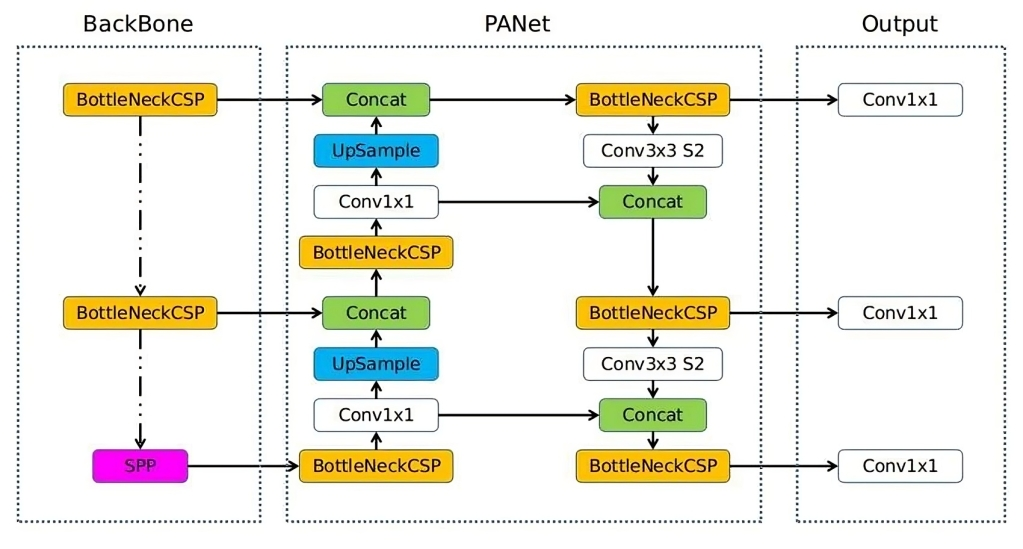
\includegraphics[scale=0.35]{Yolov5.png}}
\caption{Proposed Architecture}
\label{fig1}
\end{figure*}}

An automatic vision-based technique compares the identified cars to the pre-marked spaces to determine whether or not they are occupied. The suggested technique can be used for status identification of parking spaces in any parking spot because it uses manual marking, where the admin annotates each parking slot just once during setup. After this, an algorithm using the marks is used to identify whether or not a parking place is occupied. Here are the steps to explain how the proposed IPMS works:

\begin{itemize}
    \item \textbf{Step 1:}In addition to streaming live video to an NVR for archival purposes, the majority of IP cameras also make their feed available to any user via the RTSP protocol. Since IP cameras can double as parking lot monitors, they are perfect for these kinds of activities.
    \item \textbf{Step 2:} Locate every car: Instead of focusing on parking slot occupancy classification, the suggested solution seeks to improve the flexibility of parking spot detection systems by locating all vehicles. This method paves the way for the installation of high-tech features like ALPR and vehicle tracking. We guarantee real-time vehicle identification with optimal inference speeds by utilizing the YOLO v5 network design, more specifically the YOLOv5s variation. Autonomous vehicle detection in diverse settings is made possible using transfer learning instruction using the MS COCO dataset. For better feature acquisition and fusion, the design uses Feature Pyramid Network (FPN) with Path Integrated Network (PAN) components in the neck and Common Spatial Pattern (CSP) and focus frameworks in the backbone. The system can now accurately detect available parking spots in real-time, greatly expanding its usefulness and adaptability. See Figure \ref{fig1} for a visual depiction of the YoLOv5s network design, including its focus and CSP structures.
    \item \textbf{Step 3:} Making sure every slot is filled or empty: One approach relied on comparing the intersection over union (IOU) (Eq. (\ref{e1})), while the other relied on comparing the centroid, to verify the vacancy. When using the intersection-over-union (IOU) comparison technique, the intersection is located between the vehicle's boundary box and the parking slot. 
    \begin{equation}\label{e1}
        IOU = \frac{\text{Detect Result} \cap \text{Ground Truth}}{\text{Detect Result} \cup \text{Ground Truth}}
    \end{equation}
    Evaluating the middle point of every vehicle's limit box and then checking if a parking spot includes the centroid is how vacancy is tested after all the vehicles have been detected. The presence of a centroid in a parking slot indicates occupancy, whereas the absence of a centroid indicates vacantness. Our technique takes about 0.022 seconds every image, which is far quicker than previous proposed classifier-based systems. For comparison, the system put forth by Farley et al. \cite{farley2021real}and Acharya et al. \cite{acharya2018real} both require about 0.5 seconds per image. Using their respective IDs, a record is also created for both occupied and unoccupied parking slots.
    \item \textbf{Step 4:} Post-processing: By averaging the results across a given number of images then contrasting them with a cutoff point, post-processing ensures that any false positives are removed. The state of an area for parking is acquired by using Eq. \ref{e2} after the age that particular slot is increased for the appropriate amount of frames when a vehicle is discovered to be inside it.
    \begin{equation}\label{e2}
        Parking status = \frac{\text{Age of slot}}{\text{Specified No. of Slots}} \geq threshold
    \end{equation}
    A slot's age is simply a tally of the number of frames a vehicle spent in that slot; the detection threshold determines, for a given number of frames, the age of slot is accurate for marking that slot as occupied. The optimal trade-off for accuracy was found in real-time experiments with a detection threshold value of 0.6.
    \item \textbf{Step 5:} Analyze the results:A parking spot is assigned based on the number of instances of occupied and unoccupied slots in the record that is generated.
\end{itemize}
Figure 3 illustrate the entire process of the suggested system that may identify empty or filled slots.

\textbf{\begin{figure}[htbp]
\centerline{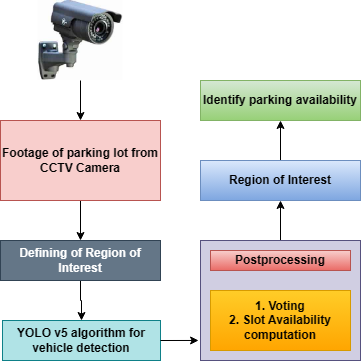
\includegraphics[width=0.35\textwidth]{WorkflowProposed.drawio.png}}
\caption{Proposed System Architecture}
\label{fig}
\end{figure}}

\section{Result Analysis}\label{sec4}
An Intel Core i7 @ 3.2 GHz CPU, with an Nvidia GTX 1050ti GPU are the components that make up the proposed system. The model was implemented using the PyTorch framework in Python, which makes use of CUDA.

We used the standard PKLot dataset to train our YOLOV5 model and then tested it. If you're having trouble telling whether a parking spot is available or not due to factors like lighting, angle of view, or weather, the PKLot dataset has you covered. Totaling 12,416 photos, the dataset is divided into three groups: training, validation, and test. The training set contains 8691 images, the validation set contains 2483 images, and the test set contains 1242 images. The ratio of these sets is 70:20:10. The best outcome on the dataset is achieved by training the YOLOv5s model on several parameter settings. Table \ref{tab1} lists the network's hyper-parameter settings.

\begin{table}[h!]
    \centering
    \caption{Hyperparameter Setting of Proposed method}
    \label{tab1}
    \begin{tabular}{|l|c|} \hline
    \textbf{Parameter} & \textbf{Value} \\ \hline
    Batch size & 32, 64 \\ \hline
    Learning rate & 0.001 \\ \hline
    Optimizer & Adam \\ \hline
    Weight decay & 0.0005 \\ \hline
    Momentum & 0.937 \\ \hline
    \end{tabular}
\end{table}

\subsection{Performance Metrics}
Performance metrics like Correct Classification Rate (CCR) or Accuracy $A_{cc}$, precision $P_{re}$, recall $R_{ec}$, and f-measure $ F1_{measure}$ are used to evaluate the effectiveness of the proposed technique. They are represented mathematically by equations \ref{eq10} to \ref{eq13}.

\begin{eqnarray}\label{eq10}
    A_{cc} & = & \frac{Tr^{Po} + Ts^{Ne}}{Tr^{Po} + Tr^{Ne}+Fa^{Po}+Fa^{Ne}} \\
    P_{re} & = & \frac{Tr^{Po}}{Tr^{Po}+Fr^{Po}} \\
    R_{ec} & = & \frac{Tr^{Po}}{Tr^{Po}+Fa^{Ne}} \\ \label{eq13}
    F1_{measure} & = & \frac{2 \times P_{re} \times R_{ec}}{P_{re} + R_{ec}}
\end{eqnarray}

The examples that were correctly classified as positive are represented by $Tr^{Po}$. Cases that were mislabeled as negative are denoted by $Tr^{Ne}$. False positives, or cases that were incorrectly classified as positive, are represented by $Fa^{Po}$. False negatives, or cases incorrectly classified as negative, are represented by the symbol $Fa^{Ne}$.

\textbf{Root Mean Squared Error (RMSE):} RMSE is a statistical measure that assesses the typical size of the discrepancies between the actual and projected values in a regression model. Bigger mistakes are punished more severely than little ones. Mathematically, RMSE expressed as 
\begin{equation}
    RSME = \sqrt{\frac{1}{n} \sum_{i=1}^n (\hat{y}_i - y_i)^2}
\end{equation}
\textbf{Mean Absolute Error (MAE):} Regardless of the direction (positive or negative), MAE calculates the mean value for the errors between projected and actual values. Compared to RMSE, it offers an error measure that is easier to understand. Mathematically, MAE represented as 
\begin{equation}
    MAE = \frac{1}{n} \sum_{i=1}^n |\hat{y}_i - y_i|
\end{equation}
Similarly, Mean Occupancy Error (MOE) is expressed as 
\begin{equation}
    MOE = \frac{1}{n} \sum_{i=1}^n \frac{|\hat{y}_i - y_i|}{\text{Number of slots}}
\end{equation}
\subsection{Experimental Results}
The network was tested using the standards PKLot dataset to see how well it could recognize the parking lot's state.

\textbf{\begin{figure}[htbp]
\centerline{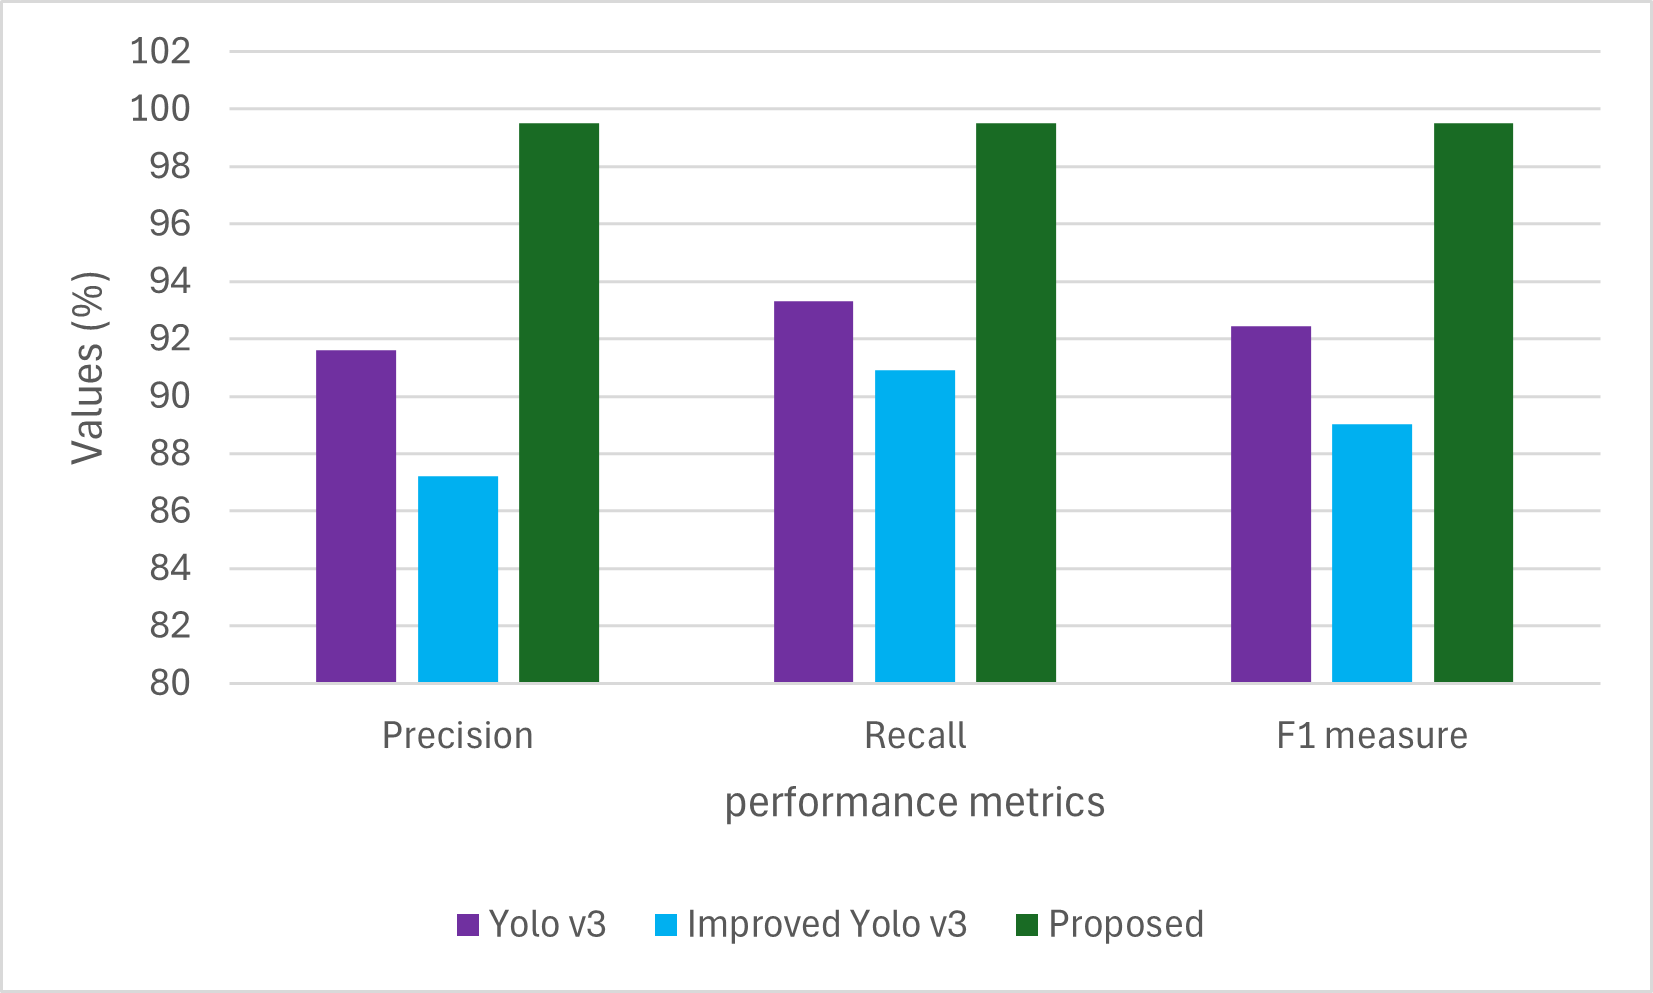
\includegraphics[width=0.5\textwidth]{Picture1.png}}
\caption{Performance metrics comparison}
\label{fig2}
\end{figure}}

Figure \ref{fig2} and Figure \ref{fig3} displays its performance using models that were previously used to categorize parking spaces. As can be seen, our network delivers cutting edge performance with the bonus of being able to integrate IPMS's more sophisticated functions, such as automatic billing, number plate recognition, and vehicle tracking.

\textbf{\begin{figure}[htbp]
\centerline{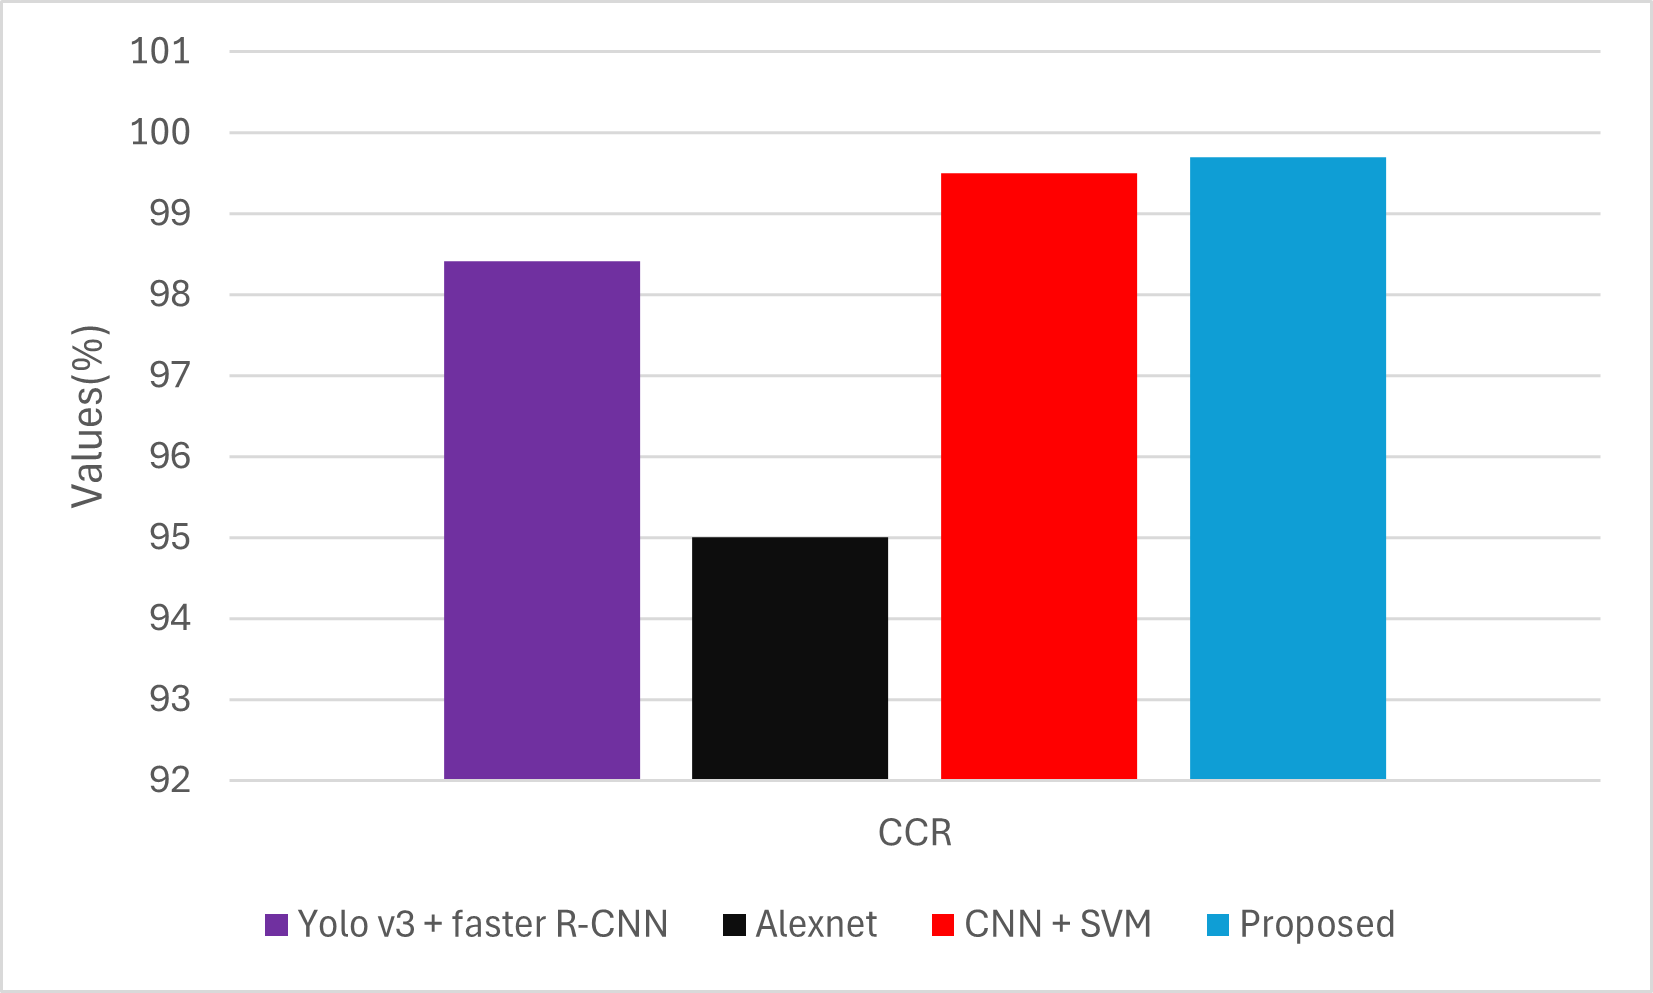
\includegraphics[width=0.45\textwidth]{Picture2.png}}
\caption{Performance comparison with other models}
\label{fig3}
\end{figure}}

Fig. \ref{fig5} illustrates that the effectiveness of the algorithms trained on the PKLot dataset degrades in real time because it lacks a consistent record of the region that is relevant and the camera direction is constant across all photos. Fig. 10 shows that, despite the model being trained with high parameter settings to enhance its performance in a live environment, the model trained on PKLot has anomalies in detected boundaries and is unable to adjust to changes in the direction and scale of the camera feed.

\textbf{\begin{figure}[htbp]
\centerline{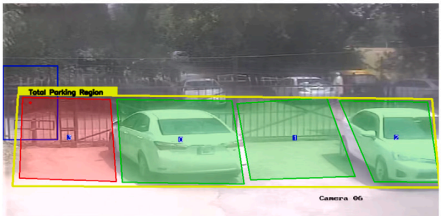
\includegraphics[width=0.5\textwidth]{Picture3.png}}
\caption{Performance of the network trained on custom dataset and PKLot dataset on live cameras.}
\label{fig5}
\end{figure}}

Using a pretrained YOLOV5s model, we were able to identify vacant parking lots in real time, which was a significant improvement over previous efforts. With an input image resolution of 640 × 640, YOLOv5s boasts 16.5 billion FLOPs, and the pre-trained model attained a MAP of 37.2 on the MS COCO datasets. The computer was able to operate at roughly 45 frames per second using an Intel Core i7. Pre-trained YOLO v5 and YOLO v5 models trained on PKLot are tested for generalisation capabilities using unseen data collected from the live feed of four cameras positioned in different positions with variable orientations and illumination conditions. As seen in Figure \ref{fig4}, the pre-trained model demonstrated superior performance compared to the PKLot-trained method. The inability of the PKLot-trained model to handle real-time problems is highlighted by the fact that its performance drops significantly when applied to live stream. The algorithm was put through its paces on both our proprietary test dataset and many real-time settings.

\textbf{\begin{figure}[htbp]
\centerline{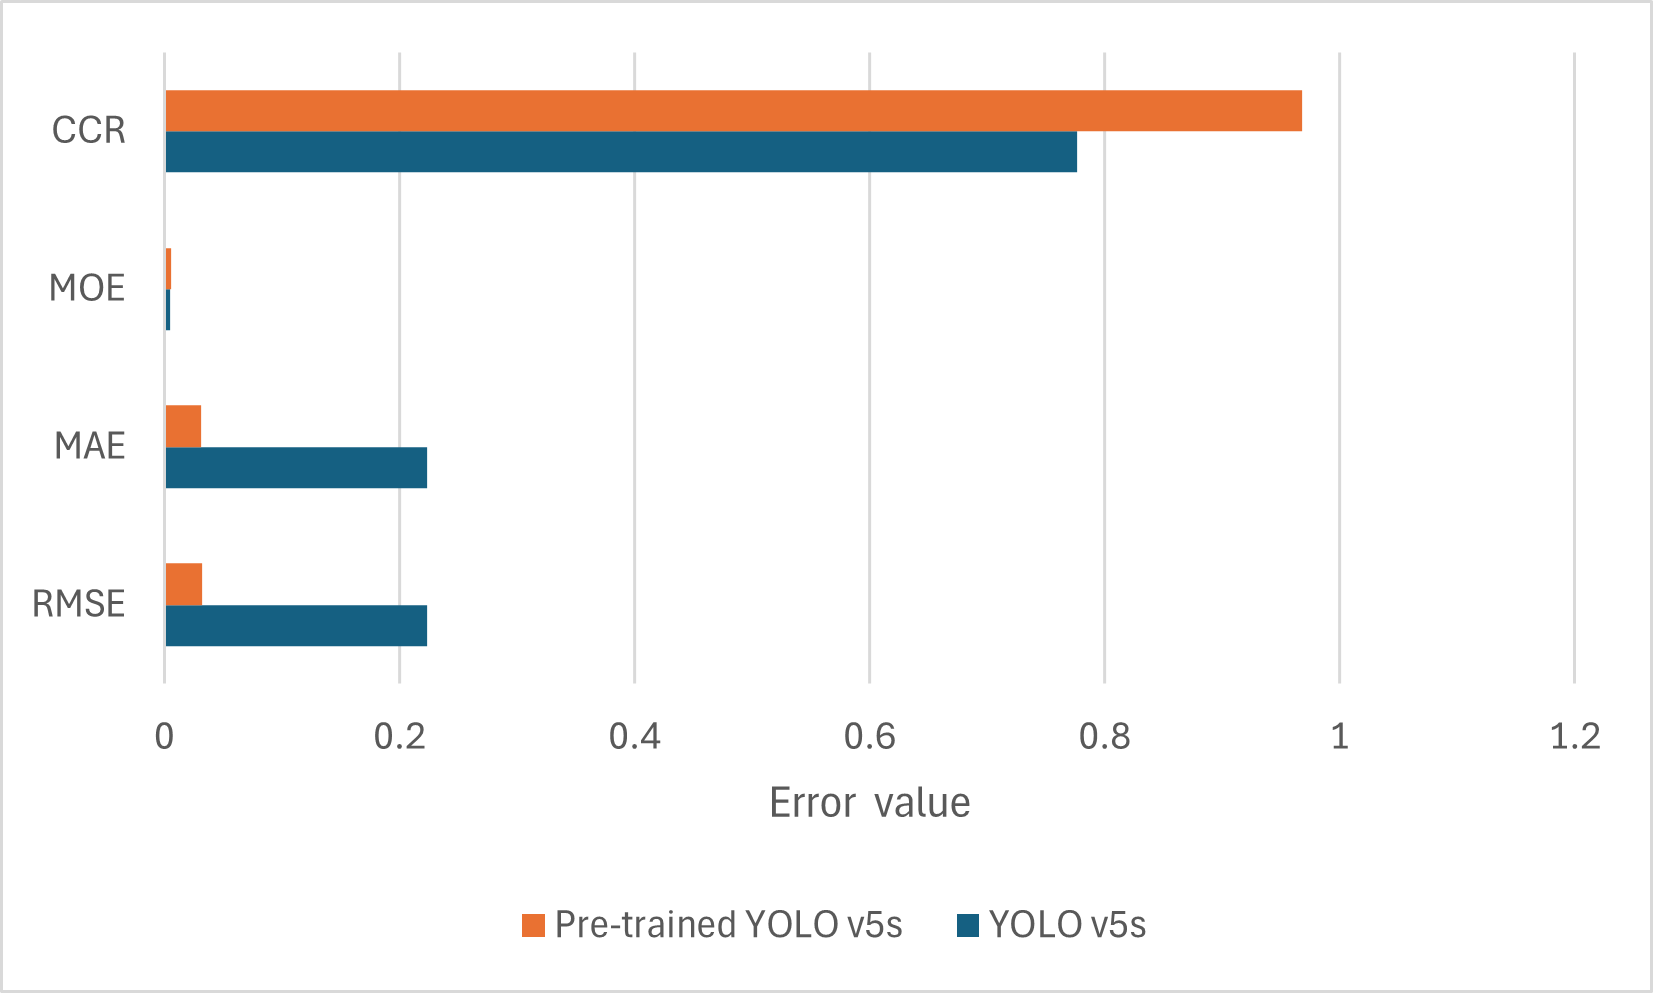
\includegraphics[width=0.45\textwidth]{Picture4.png}}
\caption{Evaluate our algorithms in a live environment}
\label{fig4}
\end{figure}}

We were able to implement the method on any parked region with varied view angles and scale—even ones without road surface marking—by manually labeling the parking spots. Red was used to identify the occupied spaces and green to highlight the vacant ones. Table \ref{fig6} shows that our model that has been trained achieves a 96.8\% success rate when faced with real-time problems.

\textbf{\begin{figure}[htbp]
\centerline{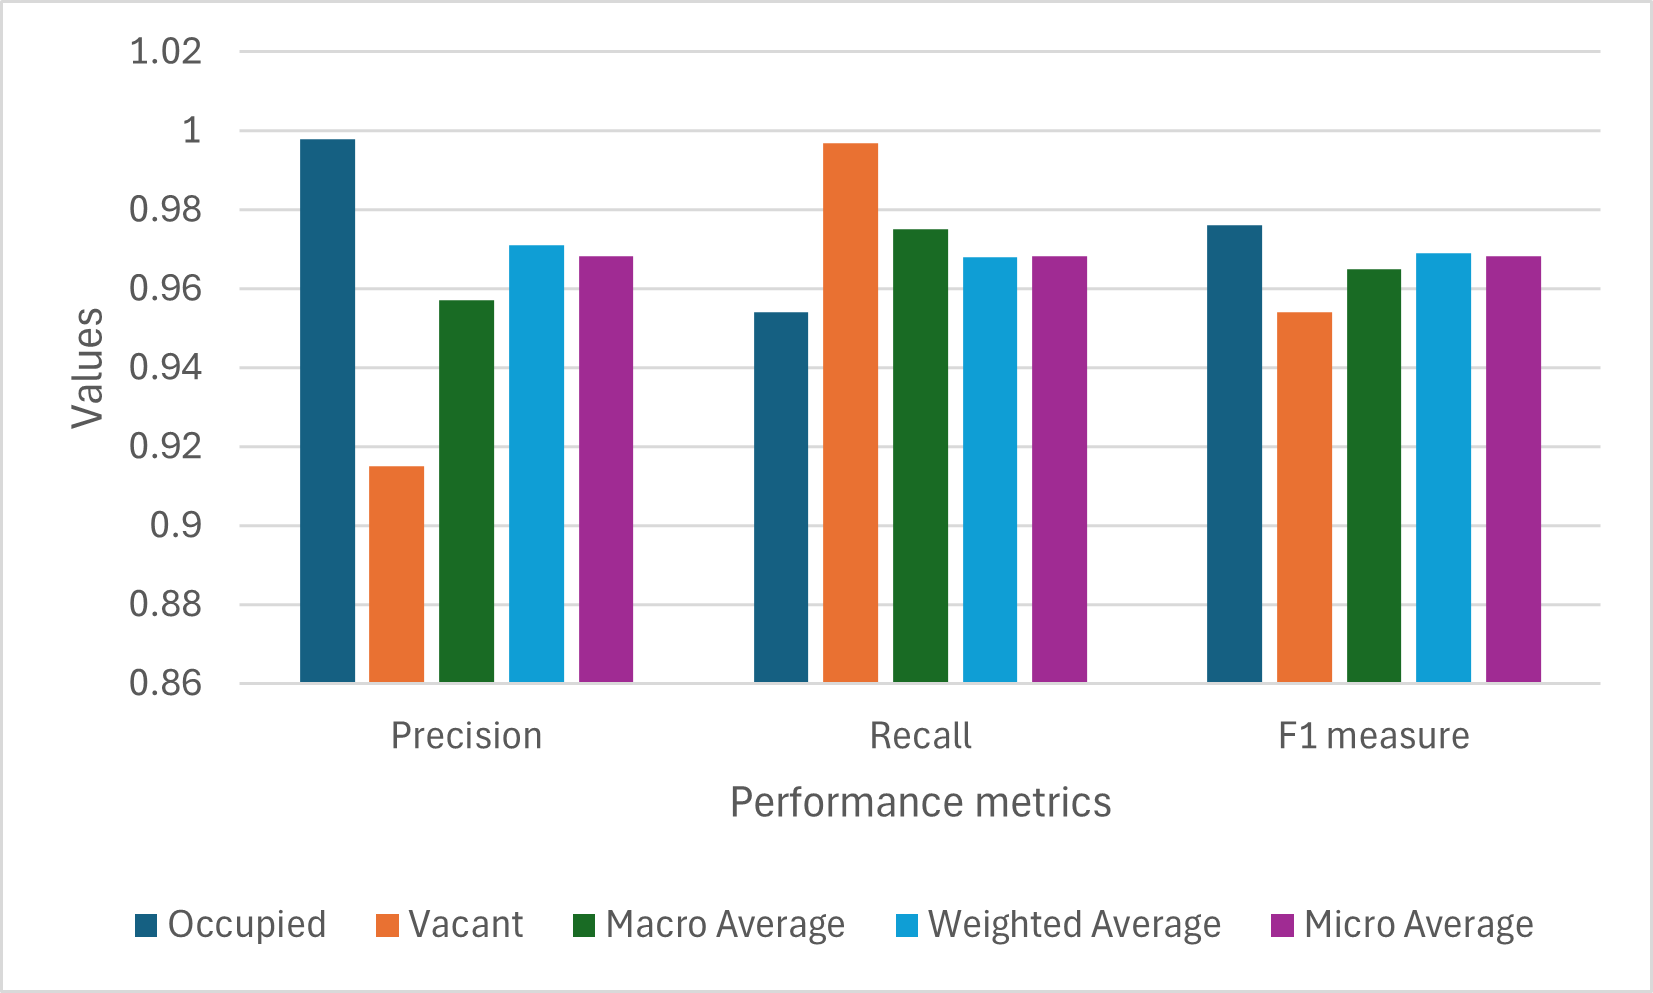
\includegraphics[width=0.45\textwidth]{Picture5.png}}
\caption{Application of pre-trained algorithm to a unique dataset for assessment.}
\label{fig6}
\end{figure}}

It is clear from Fig. \ref{fig7} that our system performs admirably on the top feed with a time frame for processing of only 0.022 seconds per image, and it also works well on feeds received from cameras with varying orientations, sizes, and lighting conditions. The network is able to distinguish between various lighting conditions, as shown in Figure \ref{fig7} in turn. Since the majority of parking lots currently have cameras installed in elevated angles, our system can be used in real time and is also scalable, cost-effective, and has a low inference time.

\textbf{\begin{figure}[htbp]
\centerline{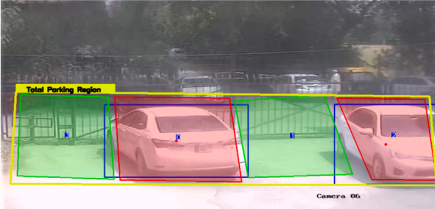
\includegraphics[width=0.5\textwidth]{Picture6.png}}
\caption{Application of pre-trained algorithm to a unique dataset for assessment.}
\label{fig7}
\end{figure}}

\section{Conclusion and future work}\label{sec5}
The integration of YOLO v5 into parking management systems represents a transformative step in addressing urban parking congestion and inefficiency. By leveraging real-time object detection and deep learning, our framework revolutionizes parking management, enabling proactive decision-making for drivers and reducing search times and congestion. The optimization of parking operations enhances overall efficiency and aligns with smart city goals of sustainability and transportation optimization. Scalable, adaptable, and integrable with existing infrastructure, our framework lays the groundwork for smarter, user-friendly parking systems. Moving forward, continued research and development will refine the framework's capabilities, including accuracy, scalability, and integration with emerging technologies like connected vehicles. In summary, the "Enhancing Parking Management Efficiency through YOLO v5" framework offers a promising solution to urban parking challenges, creating more intelligent, responsive, and sustainable parking systems for the benefit of drivers and cities alike.

In future, addressing security and privacy concerns associated with the deployment of AI-based parking management systems, including data protection, access control, and mitigation of potential security vulnerabilities. Implementing robust encryption, authentication, and anonymization techniques to safeguard sensitive information collected from parking sensors and surveillance cameras.

\bibliographystyle{IEEEtran} 
\bibliography{References.bib}
\end{document}
